\section{The optimal Clustering Method} \label{sec:Comparison_Clustering}

To further investigate in the source of the errors \autoref{fig:PCA_Cluster_Knee_4} \textbf{\textsf{B}} and \textbf{\textsf{D}}, \gls{HDBSCAN} was performed in a more simple manner, without $\varepsilon$ exploration on the small subsets of H13 and H16 of segment 4. Three different input matrices were used to compare the clustering by \gls{HDBSCAN}. The first input was the non-reduced set of k-mer freqency vectors used in \autoref{sec:K_mer_Representation} as precalculated matrix with cosine distance (\autoref{sec:MAFFT}). Clustering was then performed and the result visualized as a cluster-tree (\autoref{fig:Simple_Clustertree_Cosine}). 

\begin{figure}[!hbt]
    \centering
    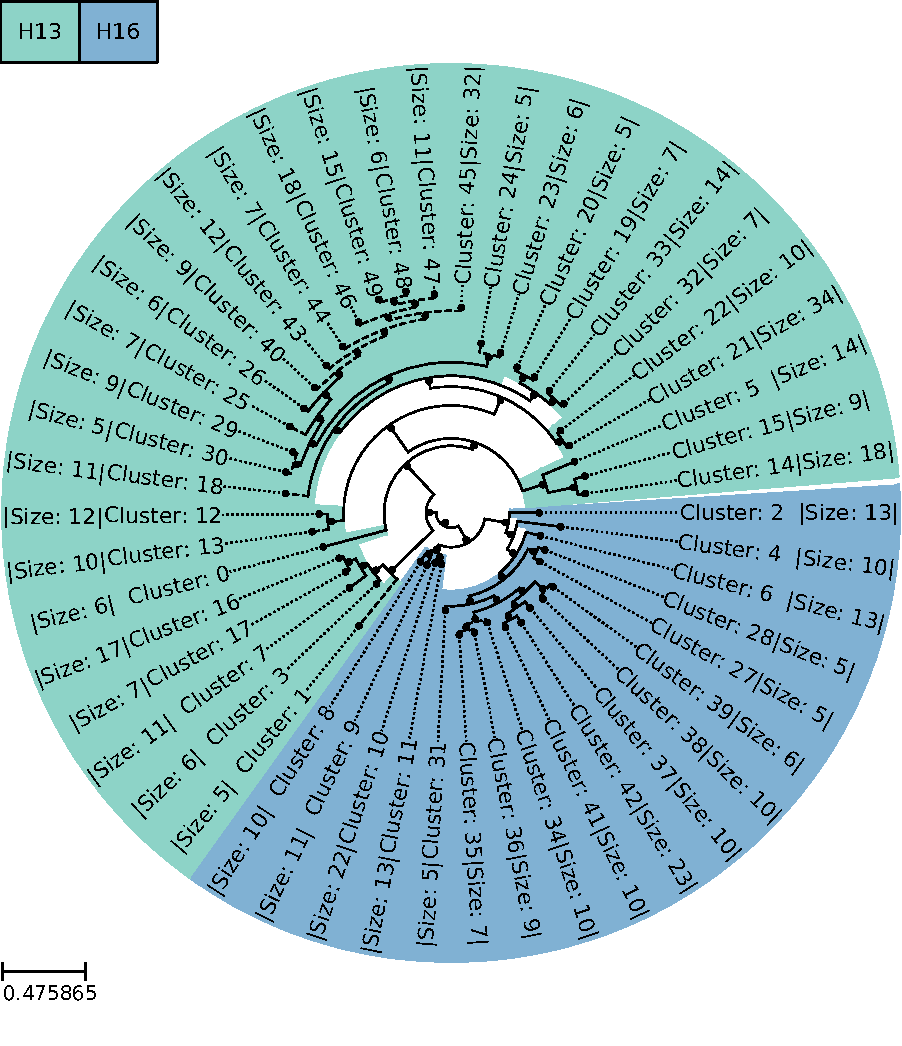
\includegraphics[width=\textwidth]{PCA/Clustertree_Segment_4_H_Cosine.pdf}
    \caption[H13/H16 Simple Clustering Example with Precalculated (cosine)]{\textbf{H13/H16 Simple Clustering Example with Precalculated (cosine).} .}
    \label{fig:Simple_Clustertree_Cosine}
\end{figure}

In a similar manner to the precalculated \gls{UPGMA}-tree in \autoref{fig:Precalculated_Cosine} the subtypes are completely separated and split on both sides in two subgroups. This points to the fact, that the clustering of the precalculated cosine distances of the k-mer frequencies are as usable as the k-mer frequencies itself and are able to draw a clear line to separate the subtypes. This finding is in line with the second simple cluster-tree based on the evolutionary distances of a \gls{MSA} containing the sequences of H13 and H16 of segment 4 (\autoref{fig:Simple_Clustertree_MSA}). The same separation is even more obvious, as the subtypes are farther away from the separation at the trees root. On the side of the H13 sequences a subdivision is also as clear as the subtype separation. Subgroups in the H16 sequences are on the other hand not that clear in \autoref{fig:Simple_Clustertree_MSA}. Maybe the different distances between the subtypes and the subgroups on each side of the subtypes is different, because evolutionary aspects like weightings and different costs for nucleotides that are more likely to change are used. In the k-mer frequencies the pure constellation of nucleotides is used, evolutionary aspects are neglected.  

\begin{figure}[!hbt]
    \centering
    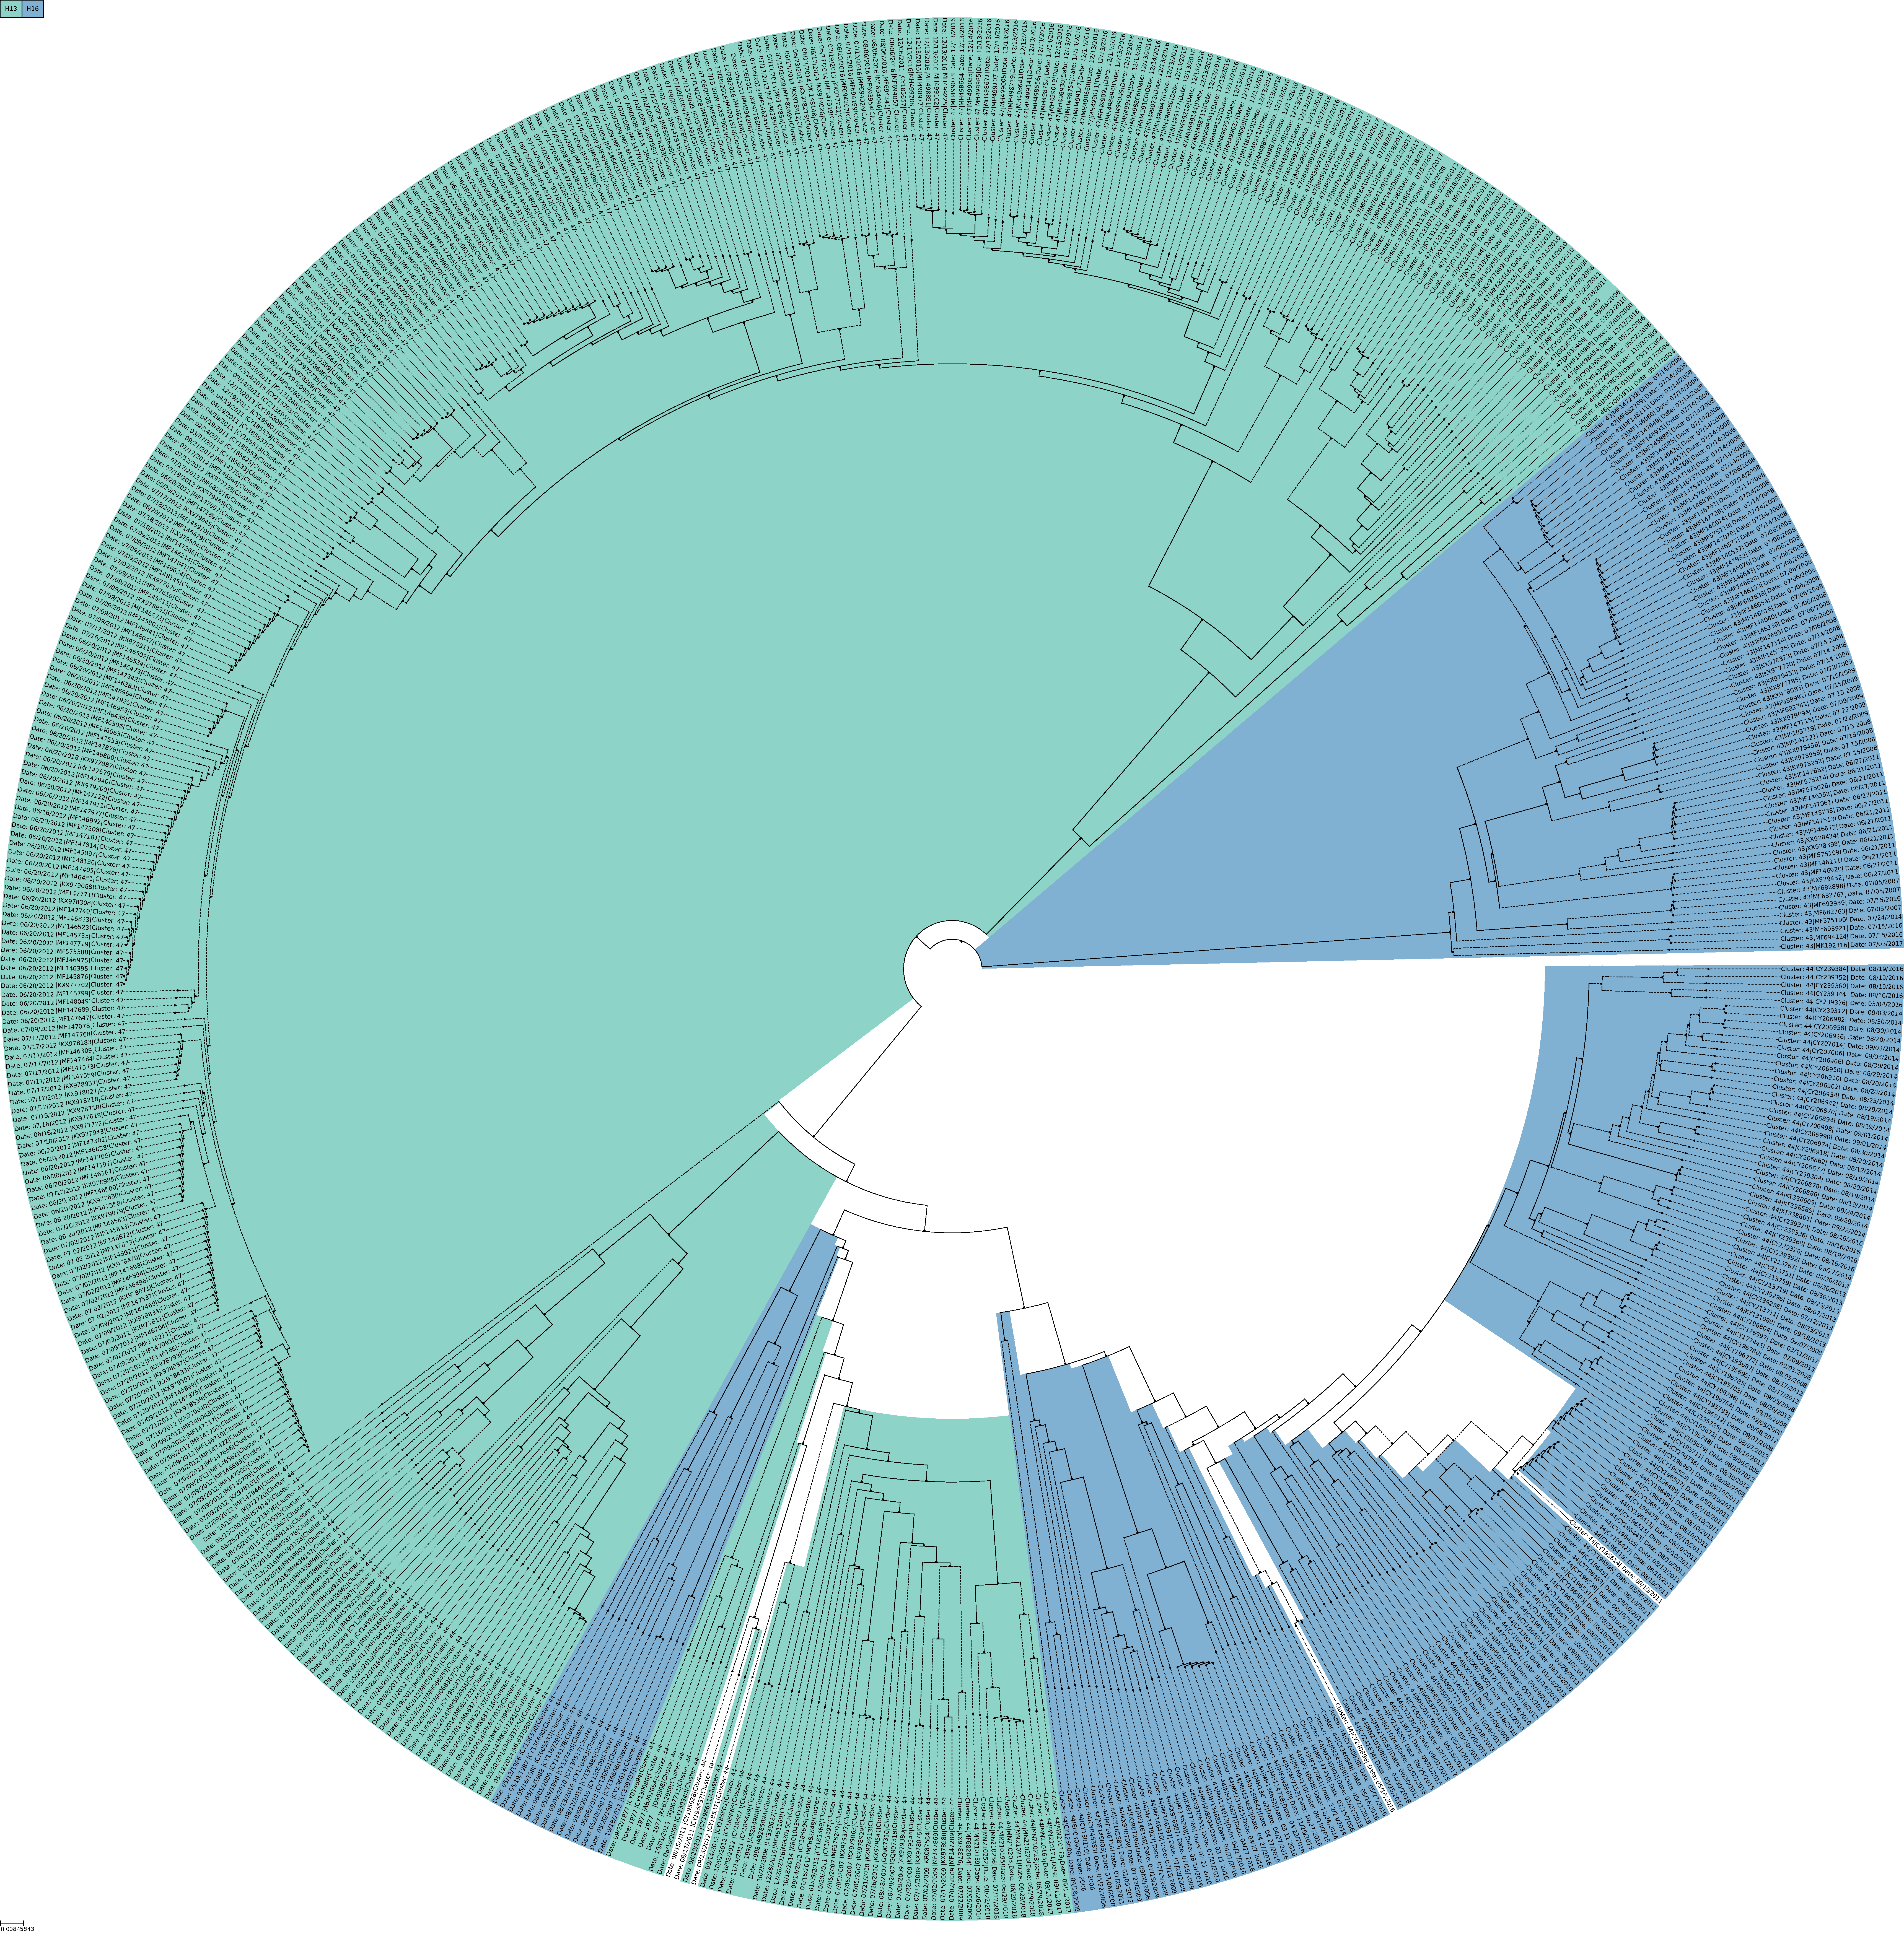
\includegraphics[width=\textwidth]{PCA/Clustertree_Segment_4_H_Focus.pdf}
    \caption[H13/H16 Simple Clustering Example with Guidetree]{\textbf{H13/H16 Simple Clustering Example with Guidetree.} .}
    \label{fig:Simple_Clustertree_MSA}
\end{figure}

\begin{figure}[!hbt]
    \centering
    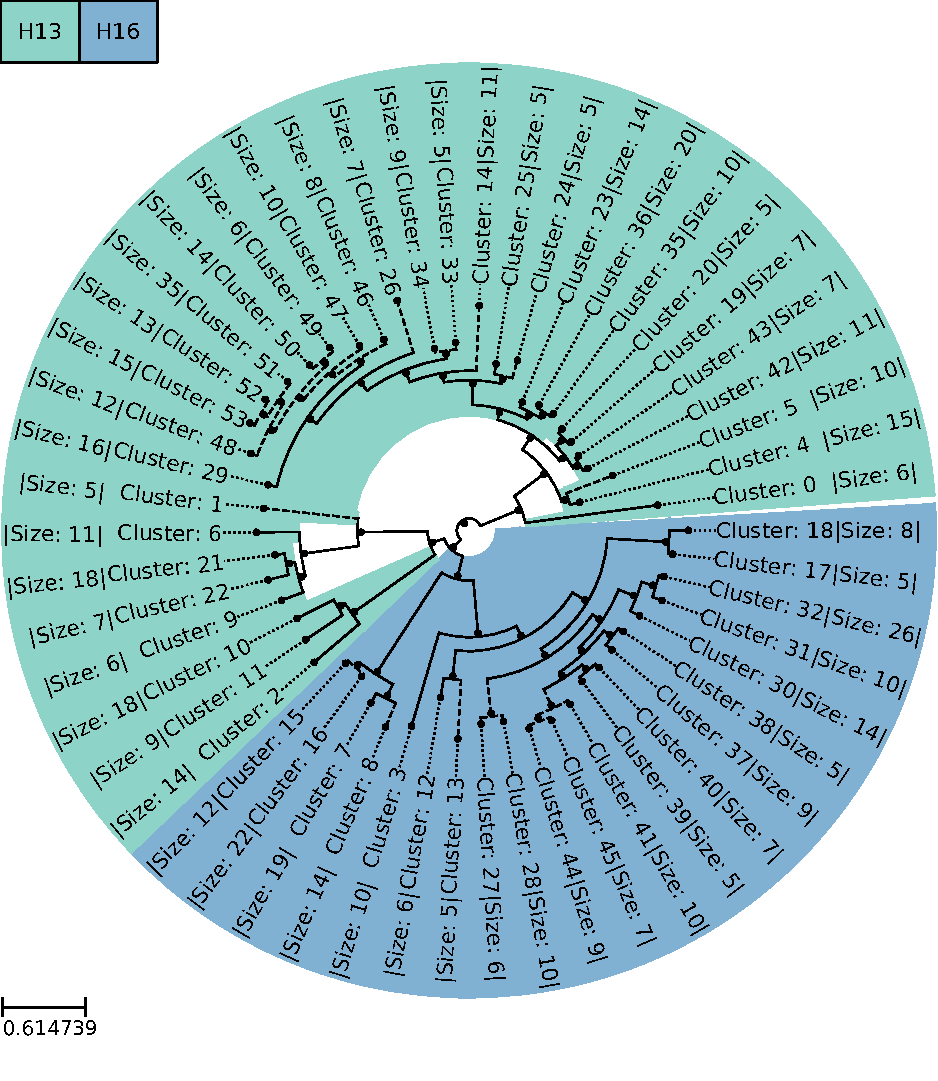
\includegraphics[width=\textwidth]{PCA/Clustertree_Segment_4_H_Simple.pdf}
    \caption[H13/H16 Simple Clustering Example (\Acrshort{PCA})]{\textbf{H13/H16 Simple Clustering Example (\Acrshort{PCA}).} .}
    \label{fig:Simple_Clustertree_PCA}
\end{figure}

As the same simple clustering and tree creation was also used on the H13 and H16 subset of the \gls{PCA} reduced vectors, the same clustering behavior as in the complete cluster-tree can be observed as no clear separation on the H13 and H16 clusters is present (\autoref{fig:Simple_Clustertree_PCA} and \autoref{fig:PCA_Clusteree_Knee_4} \textbf{\textsf{B}}). The simple clustering performed with \gls{MSA} distances and precalculated cosine distances showed a clear seperation on the subtypes. Since the prcalculated distances are solely based on the k-mer frequencies and the \gls{MSA} distances on the evolutionary aspect and both methods present a clar separation, the \gls{PCA} or dimension reduction step seems to be the origin of the clustering error in \autoref{fig:PCA_Cluster_Knee_4} \textbf{\textsf{B}} and \textbf{\textsf{D}}. The simple clustering was also performed with the same subset of H13 and H16 sequences reduced with \gls{UMAP} and can be found in the \autoref{chap:Appendix} with the precalculated simple cluster-tree that was also calculated for euclidean distance.